\documentclass[11pt,letterpaper]{article}

% =============================================================================
% PACKAGES
% =============================================================================
\usepackage[margin=1in]{geometry}
\usepackage{enumitem}
\usepackage{setspace}
\usepackage{graphicx}
\usepackage{xcolor}
\usepackage{tikz}
\usetikzlibrary{shapes.geometric, arrows.meta, positioning, fit, backgrounds, calc, decorations.pathreplacing, trees, matrix, shapes.multipart, shapes.symbols, shadows, calendar}
\usepackage{tcolorbox}
\usepackage{booktabs}
\usepackage{longtable}
\usepackage{array}
\usepackage{tabularx}
\usepackage{multirow}
\usepackage{colortbl}
\usepackage{fancyhdr}
\usepackage{titlesec}
\usepackage[colorlinks=true,linkcolor=blue!60!black,urlcolor=blue!60!black,citecolor=blue!60!black]{hyperref}
\usepackage{bookmark}
\usepackage{parskip}
\usepackage{float}
\usepackage{caption}
\usepackage{subcaption}
\usepackage{listings}
\usepackage{microtype}
\usepackage{textcomp}
\usepackage{amssymb}
\usepackage{amsmath}
\usepackage{pifont}

% =============================================================================
% CONFIGURATION
% =============================================================================
\setstretch{1.15}

% Define colors
\definecolor{primary}{RGB}{100, 60, 120}
\definecolor{secondary}{RGB}{130, 90, 150}
\definecolor{accent}{RGB}{220, 140, 60}
\definecolor{success}{RGB}{70, 150, 100}
\definecolor{warning}{RGB}{230, 180, 70}
\definecolor{critical}{RGB}{200, 80, 80}
\definecolor{lightgray}{RGB}{245, 245, 245}
\definecolor{darkgray}{RGB}{80, 80, 80}
\definecolor{teamcolor}{RGB}{220, 235, 255}
\definecolor{modulecolor}{RGB}{255, 240, 220}
\definecolor{milestonecolor}{RGB}{230, 255, 230}
\definecolor{riskcolor}{RGB}{255, 230, 230}
\definecolor{dependcolor}{RGB}{240, 230, 255}
\definecolor{phasecolor}{RGB}{255, 250, 220}
\definecolor{resourcecolor}{RGB}{230, 245, 255}

% Section formatting
\titleformat{\section}{\Large\bfseries\color{primary}}{\thesection}{1em}{}[\titlerule]
\titleformat{\subsection}{\large\bfseries\color{secondary}}{\thesubsection}{1em}{}
\titleformat{\subsubsection}{\normalsize\bfseries\color{darkgray}}{\thesubsubsection}{1em}{}

% Header/Footer
\pagestyle{fancy}
\fancyhf{}
\fancyhead[L]{\small\textcolor{darkgray}{Planner's View Specification}}
\fancyhead[R]{\small\textcolor{darkgray}{Architecture Documentation}}
\fancyfoot[C]{\thepage}
\renewcommand{\headrulewidth}{0.4pt}

% Custom environments
\newtcolorbox{definitionbox}[1][]{
    colback=lightgray,
    colframe=primary,
    fonttitle=\bfseries,
    title=#1,
    boxrule=0.5pt,
    arc=2pt,
    left=8pt,
    right=8pt,
    top=6pt,
    bottom=6pt
}

\newtcolorbox{examplebox}[1][]{
    colback=white,
    colframe=secondary,
    fonttitle=\bfseries,
    title=#1,
    boxrule=0.5pt,
    arc=2pt,
    left=8pt,
    right=8pt,
    top=6pt,
    bottom=6pt
}

\newtcolorbox{warningbox}[1][]{
    colback=orange!5,
    colframe=accent,
    fonttitle=\bfseries,
    title=#1,
    boxrule=0.5pt,
    arc=2pt,
    left=8pt,
    right=8pt,
    top=6pt,
    bottom=6pt
}

\newtcolorbox{guidancebox}[1][]{
    colback=green!5,
    colframe=success,
    fonttitle=\bfseries,
    title=#1,
    boxrule=0.5pt,
    arc=2pt,
    left=8pt,
    right=8pt,
    top=6pt,
    bottom=6pt
}

\newtcolorbox{patternbox}[1][]{
    colback=blue!3,
    colframe=primary!70,
    fonttitle=\bfseries,
    title=#1,
    boxrule=0.5pt,
    arc=2pt,
    left=8pt,
    right=8pt,
    top=6pt,
    bottom=6pt
}

\newtcolorbox{planningbox}[1][]{
    colback=purple!5,
    colframe=primary,
    fonttitle=\bfseries,
    title=#1,
    boxrule=0.5pt,
    arc=2pt,
    left=8pt,
    right=8pt,
    top=6pt,
    bottom=6pt
}

\newtcolorbox{riskbox}[1][]{
    colback=red!5,
    colframe=critical,
    fonttitle=\bfseries,
    title=#1,
    boxrule=0.5pt,
    arc=2pt,
    left=8pt,
    right=8pt,
    top=6pt,
    bottom=6pt
}

\newtcolorbox{teambox}[1][]{
    colback=blue!5,
    colframe=secondary,
    fonttitle=\bfseries,
    title=#1,
    boxrule=0.5pt,
    arc=2pt,
    left=8pt,
    right=8pt,
    top=6pt,
    bottom=6pt
}

% Listings configuration
\lstset{
    basicstyle=\ttfamily\small,
    backgroundcolor=\color{lightgray},
    frame=single,
    framerule=0.5pt,
    rulecolor=\color{darkgray},
    breaklines=true,
    captionpos=b,
    tabsize=2,
    showstringspaces=false,
    numbers=left,
    numberstyle=\tiny\color{darkgray},
    numbersep=5pt,
    xleftmargin=15pt,
    keywordstyle=\color{primary}\bfseries,
    commentstyle=\color{darkgray}\itshape,
    stringstyle=\color{success}
}

% Table column types
\newcolumntype{L}[1]{>{\raggedright\arraybackslash}p{#1}}
\newcolumntype{C}[1]{>{\centering\arraybackslash}p{#1}}
\newcolumntype{R}[1]{>{\raggedleft\arraybackslash}p{#1}}

% Custom commands
\newcommand{\cmark}{\ding{51}}
\newcommand{\xmark}{\ding{55}}

% =============================================================================
% DOCUMENT BEGIN
% =============================================================================
\begin{document}

% -----------------------------------------------------------------------------
% TITLE PAGE
% -----------------------------------------------------------------------------
\hypersetup{pageanchor=false}
\begin{titlepage}
    \centering
    \vspace*{1.5cm}
    
    {\Huge\bfseries\color{primary} Planner's View\par}
    \vspace{0.5cm}
    {\Large\color{secondary} Architecture Viewpoint Specification\par}
    \vspace{0.3cm}
    {\large\color{darkgray} Work Assignment, Team Structure \& Development Planning\par}
    
    \vspace{1.2cm}
    
    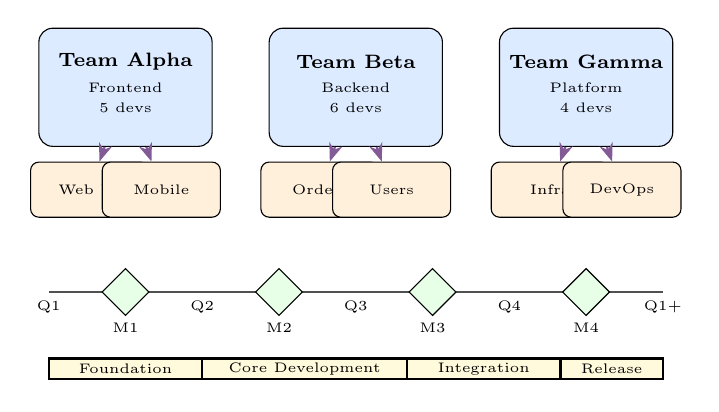
\begin{tikzpicture}[scale=0.65]
        % Teams
        \node[draw, fill=teamcolor, rounded corners=5pt, minimum width=2.2cm, minimum height=1.5cm] (team1) at (-4.5, 2.5) {};
        \node[font=\scriptsize\bfseries] at (-4.5, 3) {Team Alpha};
        \node[font=\tiny] at (-4.5, 2.5) {Frontend};
        \node[font=\tiny] at (-4.5, 2.1) {5 devs};
        
        \node[draw, fill=teamcolor, rounded corners=5pt, minimum width=2.2cm, minimum height=1.5cm] (team2) at (0, 2.5) {};
        \node[font=\scriptsize\bfseries] at (0, 3) {Team Beta};
        \node[font=\tiny] at (0, 2.5) {Backend};
        \node[font=\tiny] at (0, 2.1) {6 devs};
        
        \node[draw, fill=teamcolor, rounded corners=5pt, minimum width=2.2cm, minimum height=1.5cm] (team3) at (4.5, 2.5) {};
        \node[font=\scriptsize\bfseries] at (4.5, 3) {Team Gamma};
        \node[font=\tiny] at (4.5, 2.5) {Platform};
        \node[font=\tiny] at (4.5, 2.1) {4 devs};
        
        % Modules
        \node[draw, fill=modulecolor, rounded corners=3pt, minimum width=1.5cm, minimum height=0.7cm, font=\tiny] (m1) at (-5.2, 0.5) {Web UI};
        \node[draw, fill=modulecolor, rounded corners=3pt, minimum width=1.5cm, minimum height=0.7cm, font=\tiny] (m2) at (-3.8, 0.5) {Mobile};
        
        \node[draw, fill=modulecolor, rounded corners=3pt, minimum width=1.5cm, minimum height=0.7cm, font=\tiny] (m3) at (-0.7, 0.5) {Orders};
        \node[draw, fill=modulecolor, rounded corners=3pt, minimum width=1.5cm, minimum height=0.7cm, font=\tiny] (m4) at (0.7, 0.5) {Users};
        
        \node[draw, fill=modulecolor, rounded corners=3pt, minimum width=1.5cm, minimum height=0.7cm, font=\tiny] (m5) at (3.8, 0.5) {Infra};
        \node[draw, fill=modulecolor, rounded corners=3pt, minimum width=1.5cm, minimum height=0.7cm, font=\tiny] (m6) at (5.2, 0.5) {DevOps};
        
        % Assignments
        \draw[-{Stealth}, thick, secondary] (team1) -- (m1);
        \draw[-{Stealth}, thick, secondary] (team1) -- (m2);
        \draw[-{Stealth}, thick, secondary] (team2) -- (m3);
        \draw[-{Stealth}, thick, secondary] (team2) -- (m4);
        \draw[-{Stealth}, thick, secondary] (team3) -- (m5);
        \draw[-{Stealth}, thick, secondary] (team3) -- (m6);
        
        % Timeline
        \draw[thick, darkgray] (-6, -1.5) -- (6, -1.5);
        \node[font=\tiny] at (-6, -1.8) {Q1};
        \node[font=\tiny] at (-3, -1.8) {Q2};
        \node[font=\tiny] at (0, -1.8) {Q3};
        \node[font=\tiny] at (3, -1.8) {Q4};
        \node[font=\tiny] at (6, -1.8) {Q1+};
        
        % Milestones
        \node[draw, fill=milestonecolor, diamond, minimum size=0.6cm, font=\tiny] at (-4.5, -1.5) {};
        \node[font=\tiny] at (-4.5, -2.2) {M1};
        
        \node[draw, fill=milestonecolor, diamond, minimum size=0.6cm, font=\tiny] at (-1.5, -1.5) {};
        \node[font=\tiny] at (-1.5, -2.2) {M2};
        
        \node[draw, fill=milestonecolor, diamond, minimum size=0.6cm, font=\tiny] at (1.5, -1.5) {};
        \node[font=\tiny] at (1.5, -2.2) {M3};
        
        \node[draw, fill=milestonecolor, diamond, minimum size=0.6cm, font=\tiny] at (4.5, -1.5) {};
        \node[font=\tiny] at (4.5, -2.2) {M4};
        
        % Phase bars
        \draw[thick, fill=phasecolor] (-6, -2.8) rectangle (-3, -3.2);
        \node[font=\tiny] at (-4.5, -3) {Foundation};
        
        \draw[thick, fill=phasecolor] (-3, -2.8) rectangle (1, -3.2);
        \node[font=\tiny] at (-1, -3) {Core Development};
        
        \draw[thick, fill=phasecolor] (1, -2.8) rectangle (4, -3.2);
        \node[font=\tiny] at (2.5, -3) {Integration};
        
        \draw[thick, fill=phasecolor] (4, -2.8) rectangle (6, -3.2);
        \node[font=\tiny] at (5, -3) {Release};
        
    \end{tikzpicture}
    
    \vspace{1.3cm}
    
    \begin{tabular}{ll}
        \textbf{Version:} & 2.0 \\
        \textbf{Status:} & Release \\
        \textbf{Classification:} & ISO/IEC/IEEE 42010 Compliant \\
        \textbf{Last Updated:} & \today \\
    \end{tabular}
    
    \vfill
    
    {\small Based on the Views and Beyond approach to software architecture documentation}
    
\end{titlepage}
\clearpage
\hypersetup{pageanchor=true}

% -----------------------------------------------------------------------------
% TABLE OF CONTENTS
% -----------------------------------------------------------------------------
\tableofcontents
\newpage

% =============================================================================
% SECTION: VIEWPOINT NAME
% =============================================================================
\section{Viewpoint Name}

\begin{definitionbox}[Viewpoint Identification]
\begin{tabular}{@{}L{3.5cm}L{10cm}@{}}
\textbf{Name:} & Planner's View \\[0.5em]
\textbf{Synonyms:} & Work Assignment View, Allocation View, Team Structure View, Project Planning View, Resource View, Development Organization View \\[0.5em]
\textbf{Identifier:} & VP-PLAN-001 \\[0.5em]
\textbf{Version:} & 2.0 \\
\end{tabular}
\end{definitionbox}

\subsection{Viewpoint Classification}

The Planner's View is an allocation-style view in the Views and Beyond approach, specifically the Work Assignment style. It maps software elements to the organizational units (teams, developers) responsible for developing and maintaining them. This viewpoint bridges architecture and project management, enabling effective planning, resource allocation, and coordination.

\begin{table}[H]
\centering
\caption{Viewpoint Classification Taxonomy}
\begin{tabular}{@{}L{4cm}L{10cm}@{}}
\toprule
\textbf{Attribute} & \textbf{Value} \\
\midrule
Style Family & Allocation Styles \\
Primary Focus & Work Assignment and Team Organization \\
Abstraction Level & Organizational / Planning \\
Temporal Perspective & Project Timeline and Phases \\
Related Styles & Work Assignment, Deployment (allocation) \\
IEEE 42010 Category & Development Viewpoint (organizational aspects) \\
Relationship & Bridges Architecture and Project Management \\
\bottomrule
\end{tabular}
\end{table}

\subsection{Viewpoint Scope}

The Planner's View encompasses the following aspects:

\begin{itemize}
    \item \textbf{Work Assignment:} Mapping of architectural elements to teams and individuals responsible for their development.
    
    \item \textbf{Team Structure:} Organization of development teams, their skills, and responsibilities.
    
    \item \textbf{Development Phases:} Timeline of project phases aligned with architectural milestones.
    
    \item \textbf{Resource Allocation:} Assignment of personnel, time, and budget to work items.
    
    \item \textbf{Dependencies and Sequencing:} Order in which work must be performed based on architectural dependencies.
    
    \item \textbf{Risk Management:} Technical and organizational risks affecting development.
    
    \item \textbf{Effort Estimation:} Estimates for developing architectural elements.
    
    \item \textbf{Communication Paths:} Required coordination between teams based on element interactions.
\end{itemize}

% =============================================================================
% SECTION: OVERVIEW
% =============================================================================
\section{Overview}

The Planner's View provides essential information for project planning and management by connecting architectural structure to development organization. It ensures that the technical architecture and organizational structure are aligned for effective delivery.

\subsection{Purpose and Scope}

The primary purpose of this viewpoint is to enable project managers, architects, and team leads to plan and coordinate development activities based on the system's architectural structure. It answers questions about who builds what, when, and how work is coordinated across teams.

\begin{definitionbox}[Viewpoint Definition]
The Planner's View maps software architecture elements to organizational units (teams, roles, individuals) and project timeline elements (phases, milestones, iterations). It documents work assignments, team structures, development sequences, resource allocations, and coordination requirements, providing the foundation for effective project planning and execution.
\end{definitionbox}

\subsection{Key Characteristics}

The Planner's View exhibits several distinctive characteristics:

\textbf{Allocation Focus:} Maps architectural elements to organizational and temporal elements, bridging technical and management domains.

\textbf{Conway's Law Awareness:} Recognizes that system structure and team structure influence each other and should be aligned.

\textbf{Dynamic Nature:} Updates as project progresses, teams change, and architectural understanding evolves.

\textbf{Multi-Stakeholder:} Serves both technical (architects, developers) and management (PMs, resource managers) audiences.

\textbf{Planning Foundation:} Provides the structural basis for project schedules, resource plans, and coordination strategies.

\subsection{Relationship to Other Viewpoints}

The Planner's View connects to other architectural viewpoints:

\begin{table}[H]
\centering
\caption{Relationships to Other Viewpoints}
\begin{tabular}{@{}L{3.5cm}L{10.5cm}@{}}
\toprule
\textbf{Viewpoint} & \textbf{Relationship} \\
\midrule
Development & Module structure determines work breakdown. Package ownership maps to team assignments. \\
\addlinespace
Logical & Domain boundaries inform team boundaries (inverse Conway). Service ownership by teams. \\
\addlinespace
Deployment & Deployment units may align with team responsibilities. Ops teams for infrastructure. \\
\addlinespace
Component-and-Connector & Runtime components map to developing/maintaining teams. \\
\addlinespace
Context & External integrations require coordination with external parties. \\
\addlinespace
Process & Complex concurrency may require specialized team skills. \\
\bottomrule
\end{tabular}
\end{table}

\subsection{Planning Architecture Overview}

\begin{figure}[H]
\centering
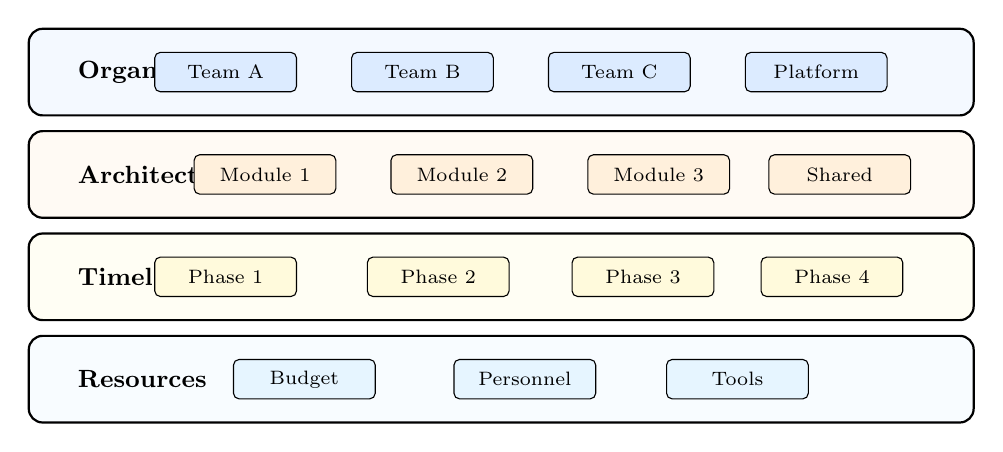
\begin{tikzpicture}[
    node distance=1cm and 1.5cm,
    layer/.style={draw, thick, rounded corners=5pt, minimum width=12cm, minimum height=1.1cm, font=\small},
    element/.style={draw, fill=teamcolor, rounded corners=2pt, minimum width=1.8cm, minimum height=0.5cm, font=\scriptsize},
]
    % Layers
    \node[layer, fill=teamcolor!30] (org) at (0, 3.5) {};
    \node[font=\small\bfseries, anchor=west] at (-5.5, 3.5) {Organization};
    
    \node[layer, fill=modulecolor!30] (arch) at (0, 2.2) {};
    \node[font=\small\bfseries, anchor=west] at (-5.5, 2.2) {Architecture};
    
    \node[layer, fill=phasecolor!30] (timeline) at (0, 0.9) {};
    \node[font=\small\bfseries, anchor=west] at (-5.5, 0.9) {Timeline};
    
    \node[layer, fill=resourcecolor!30] (resources) at (0, -0.4) {};
    \node[font=\small\bfseries, anchor=west] at (-5.5, -0.4) {Resources};
    
    % Organization elements
    \node[element] at (-3.5, 3.5) {Team A};
    \node[element] at (-1, 3.5) {Team B};
    \node[element] at (1.5, 3.5) {Team C};
    \node[element] at (4, 3.5) {Platform};
    
    % Architecture elements
    \node[element, fill=modulecolor] at (-3, 2.2) {Module 1};
    \node[element, fill=modulecolor] at (-0.5, 2.2) {Module 2};
    \node[element, fill=modulecolor] at (2, 2.2) {Module 3};
    \node[element, fill=modulecolor] at (4.3, 2.2) {Shared};
    
    % Timeline elements
    \node[element, fill=phasecolor] at (-3.5, 0.9) {Phase 1};
    \node[element, fill=phasecolor] at (-0.8, 0.9) {Phase 2};
    \node[element, fill=phasecolor] at (1.8, 0.9) {Phase 3};
    \node[element, fill=phasecolor] at (4.2, 0.9) {Phase 4};
    
    % Resource elements
    \node[element, fill=resourcecolor] at (-2.5, -0.4) {Budget};
    \node[element, fill=resourcecolor] at (0.3, -0.4) {Personnel};
    \node[element, fill=resourcecolor] at (3, -0.4) {Tools};
    
\end{tikzpicture}
\caption{Planning Architecture Layers}
\end{figure}

% =============================================================================
% SECTION: CONCERNS
% =============================================================================
\section{Concerns}

This section enumerates the architectural concerns that the Planner's View is designed to address.

\subsection{Primary Concerns}

\begin{enumerate}[label=\textbf{C\arabic*:}, leftmargin=2.5em]
    \item \textbf{Work Assignment}
    \begin{itemize}[nosep]
        \item Which team is responsible for which architectural elements?
        \item What is the ownership model (single owner vs shared)?
        \item How are responsibilities distributed across teams?
        \item What happens when team composition changes?
        \item How are cross-cutting concerns assigned?
    \end{itemize}
    
    \item \textbf{Team Structure and Skills}
    \begin{itemize}[nosep]
        \item What teams exist and what are their compositions?
        \item What skills does each team possess?
        \item Are there skill gaps relative to assigned work?
        \item How are teams organized (feature, component, platform)?
        \item What is the team topology?
    \end{itemize}
    
    \item \textbf{Development Sequencing}
    \begin{itemize}[nosep]
        \item In what order must elements be developed?
        \item What are the architectural dependencies affecting sequence?
        \item What can be developed in parallel?
        \item What is the critical path?
        \item How do integration points affect sequencing?
    \end{itemize}
    
    \item \textbf{Effort Estimation}
    \begin{itemize}[nosep]
        \item How much effort is required for each element?
        \item What factors affect estimation (complexity, novelty, risk)?
        \item What estimation techniques are appropriate?
        \item How is uncertainty captured?
        \item How are estimates validated and refined?
    \end{itemize}
    
    \item \textbf{Resource Allocation}
    \begin{itemize}[nosep]
        \item How are personnel allocated to work items?
        \item What is the budget allocation across elements?
        \item Are resources sufficient for planned work?
        \item How are resource conflicts resolved?
        \item What is the resource utilization?
    \end{itemize}
    
    \item \textbf{Milestones and Phases}
    \begin{itemize}[nosep]
        \item What are the major project milestones?
        \item How do phases align with architectural increments?
        \item What deliverables are expected at each milestone?
        \item How is progress measured?
        \item What are the release criteria?
    \end{itemize}
    
    \item \textbf{Team Coordination}
    \begin{itemize}[nosep]
        \item Which teams need to coordinate?
        \item What interfaces exist between team responsibilities?
        \item How is cross-team communication managed?
        \item What synchronization points exist?
        \item How are integration activities coordinated?
    \end{itemize}
    
    \item \textbf{Risk Management}
    \begin{itemize}[nosep]
        \item What technical risks affect planning?
        \item What organizational risks exist?
        \item What dependencies create risk?
        \item How are risks mitigated in the plan?
        \item What contingency exists?
    \end{itemize}
    
    \item \textbf{Knowledge and Learning}
    \begin{itemize}[nosep]
        \item What knowledge is required for each element?
        \item Where does expertise reside?
        \item What training is needed?
        \item How is knowledge transferred?
        \item What documentation supports handoff?
    \end{itemize}
    
    \item \textbf{Evolution and Maintenance}
    \begin{itemize}[nosep]
        \item Who maintains elements post-delivery?
        \item How does ownership evolve over time?
        \item What is the long-term team structure?
        \item How are enhancements assigned?
        \item What is the support model?
    \end{itemize}
\end{enumerate}

\subsection{Concern-Quality Attribute Mapping}

\begin{table}[H]
\centering
\caption{Concern to Project Attribute Mapping}
\small
\begin{tabular}{@{}L{3cm}C{1.1cm}C{1.1cm}C{1.1cm}C{1.1cm}C{1.1cm}C{1.1cm}C{1.1cm}@{}}
\toprule
\textbf{Concern} & \rotatebox{60}{\textbf{Schedule}} & \rotatebox{60}{\textbf{Budget}} & \rotatebox{60}{\textbf{Quality}} & \rotatebox{60}{\textbf{Velocity}} & \rotatebox{60}{\textbf{Predict.}} & \rotatebox{60}{\textbf{Agility}} & \rotatebox{60}{\textbf{Risk}} \\
\midrule
Work Assignment & $\circ$ & $\circ$ & $\bullet$ & $\bullet$ & $\circ$ & $\circ$ & $\circ$ \\
Team Structure & $\circ$ & $\bullet$ & $\bullet$ & $\bullet$ & $\circ$ & $\bullet$ & $\circ$ \\
Sequencing & $\bullet$ & $\circ$ & $\circ$ & $\circ$ & $\bullet$ & $\circ$ & $\bullet$ \\
Estimation & $\bullet$ & $\bullet$ & -- & $\circ$ & $\bullet$ & $\circ$ & $\circ$ \\
Resources & $\bullet$ & $\bullet$ & $\circ$ & $\bullet$ & $\circ$ & $\circ$ & $\circ$ \\
Milestones & $\bullet$ & $\circ$ & $\circ$ & $\circ$ & $\bullet$ & $\circ$ & $\circ$ \\
Coordination & $\circ$ & $\circ$ & $\bullet$ & $\circ$ & $\circ$ & $\circ$ & $\bullet$ \\
Risk Mgmt & $\bullet$ & $\bullet$ & $\circ$ & $\circ$ & $\circ$ & $\circ$ & $\bullet$ \\
Knowledge & $\circ$ & $\circ$ & $\bullet$ & $\circ$ & $\circ$ & $\bullet$ & $\bullet$ \\
Evolution & $\circ$ & $\bullet$ & $\bullet$ & $\circ$ & $\circ$ & $\bullet$ & $\circ$ \\
\bottomrule
\multicolumn{8}{l}{\footnotesize $\bullet$ = Primary impact, $\circ$ = Secondary impact, -- = Minimal impact}
\end{tabular}
\end{table}

% =============================================================================
% SECTION: ANTI-CONCERNS
% =============================================================================
\section{Anti-Concerns}

Understanding what the Planner's View is \emph{not} appropriate for helps stakeholders avoid misapplying this viewpoint.

\subsection{Out of Scope Topics}

\begin{enumerate}[label=\textbf{AC\arabic*:}, leftmargin=2.5em]
    \item \textbf{Detailed Technical Design}
    \begin{itemize}[nosep]
        \item Algorithm implementations
        \item Data structure choices
        \item API specifications
        \item Code-level patterns
        \item Technology selections (except as affects planning)
    \end{itemize}
    
    \item \textbf{Runtime Architecture}
    \begin{itemize}[nosep]
        \item Process and thread design
        \item Performance characteristics
        \item Scalability mechanisms
        \item Deployment topology
        \item Operational behavior
    \end{itemize}
    
    \item \textbf{Individual Task Management}
    \begin{itemize}[nosep]
        \item Daily task assignments
        \item Sprint-level planning details
        \item Individual developer schedules
        \item Bug tracking
        \item Code review assignments
    \end{itemize}
    
    \item \textbf{HR and Personnel Details}
    \begin{itemize}[nosep]
        \item Salary information
        \item Performance reviews
        \item Career development
        \item Hiring decisions (except capacity)
        \item Personal information
    \end{itemize}
    
    \item \textbf{Business Requirements}
    \begin{itemize}[nosep]
        \item Functional specifications
        \item User stories content
        \item Acceptance criteria
        \item Business rules
        \item Feature prioritization rationale
    \end{itemize}
\end{enumerate}

\begin{warningbox}[Common Misapplications]
Avoid using the Planner's View for:

\begin{itemize}[nosep]
    \item Detailed sprint planning (use Agile tools)
    \item Technical design decisions (use Development Viewpoint)
    \item Runtime behavior analysis (use Process/C\&C Viewpoints)
    \item Requirements management (use Requirements documents)
    \item Day-to-day task tracking (use project management tools)
\end{itemize}
\end{warningbox}

% =============================================================================
% SECTION: TYPICAL STAKEHOLDERS
% =============================================================================
\section{Typical Stakeholders}

The Planner's View serves stakeholders involved in project planning and coordination.

\subsection{Primary Stakeholders}

\begin{table}[H]
\centering
\caption{Primary Stakeholder Analysis}
\small
\begin{tabular}{@{}L{2.6cm}L{3.6cm}L{7cm}@{}}
\toprule
\textbf{Stakeholder} & \textbf{Role Description} & \textbf{Primary Interests} \\
\midrule
Project Managers & Plan and track delivery & Schedules, resources, milestones, risks, dependencies \\
\addlinespace
Software Architects & Design system structure & Work breakdown alignment, team coordination points \\
\addlinespace
Development Managers & Manage dev teams & Team assignments, capacity, skill requirements \\
\addlinespace
Team Leads & Lead development teams & Team responsibilities, dependencies, coordination \\
\addlinespace
Resource Managers & Allocate personnel & Staffing needs, skill matching, utilization \\
\addlinespace
Program Managers & Coordinate programs & Cross-project dependencies, portfolio view \\
\bottomrule
\end{tabular}
\end{table}

\subsection{Secondary Stakeholders}

\begin{table}[H]
\centering
\caption{Secondary Stakeholder Analysis}
\small
\begin{tabular}{@{}L{2.6cm}L{3.6cm}L{7cm}@{}}
\toprule
\textbf{Stakeholder} & \textbf{Role Description} & \textbf{Primary Interests} \\
\midrule
Senior Developers & Implement key elements & Understanding scope, dependencies, timeline \\
\addlinespace
Product Managers & Define product direction & Feature delivery timing, release planning \\
\addlinespace
Finance/PMO & Track budget and costs & Cost estimates, budget allocation, variance \\
\addlinespace
Executive Sponsors & Fund and oversee project & High-level progress, risks, resource needs \\
\addlinespace
QA Managers & Plan testing activities & Test planning, integration points, timelines \\
\addlinespace
External Partners & Provide integrations & Integration timelines, coordination points \\
\bottomrule
\end{tabular}
\end{table}

\subsection{Stakeholder Concern Matrix}

\begin{table}[H]
\centering
\caption{Stakeholder-Concern Responsibility Matrix}
\footnotesize
\begin{tabular}{@{}L{2cm}C{0.8cm}C{0.8cm}C{0.8cm}C{0.8cm}C{0.8cm}C{0.8cm}C{0.8cm}C{0.8cm}C{0.8cm}C{0.8cm}@{}}
\toprule
& \rotatebox{60}{\textbf{Assign.}} & \rotatebox{60}{\textbf{Teams}} & \rotatebox{60}{\textbf{Sequence}} & \rotatebox{60}{\textbf{Estimate}} & \rotatebox{60}{\textbf{Resource}} & \rotatebox{60}{\textbf{Milest.}} & \rotatebox{60}{\textbf{Coord.}} & \rotatebox{60}{\textbf{Risk}} & \rotatebox{60}{\textbf{Knowl.}} & \rotatebox{60}{\textbf{Evolve}} \\
\midrule
Project Mgr & A & C & R & A & R & R & A & R & C & C \\
Architect & R & C & R & C & C & C & R & R & A & C \\
Dev Manager & R & A & C & C & A & C & R & C & R & A \\
Team Lead & R & R & C & R & C & C & R & C & R & R \\
Resource Mgr & C & C & I & C & R & I & I & C & C & C \\
Sponsor & I & I & I & I & A & A & I & A & I & I \\
\bottomrule
\multicolumn{11}{l}{\footnotesize R = Responsible, A = Accountable, C = Consulted, I = Informed}
\end{tabular}
\end{table}

% =============================================================================
% SECTION: MODEL TYPES
% =============================================================================
\section{Model Types}

The Planner's View employs several complementary model types to capture different aspects of work assignment and planning.

\subsection{Model Type Catalog}

\begin{enumerate}[label=\textbf{MT\arabic*:}, leftmargin=2.5em]
    \item \textbf{Work Assignment Matrix}
    \begin{itemize}[nosep]
        \item \textit{Purpose:} Map architectural elements to responsible teams
        \item \textit{Primary Elements:} Elements, teams, responsibility types
        \item \textit{Key Relationships:} Owns, contributes-to, consumes
        \item \textit{Typical Notation:} RACI matrices, ownership tables
    \end{itemize}
    
    \item \textbf{Team Structure Diagram}
    \begin{itemize}[nosep]
        \item \textit{Purpose:} Show team organization and relationships
        \item \textit{Primary Elements:} Teams, roles, reporting lines
        \item \textit{Key Relationships:} Reports-to, collaborates-with
        \item \textit{Typical Notation:} Org charts, team topology diagrams
    \end{itemize}
    
    \item \textbf{Development Timeline}
    \begin{itemize}[nosep]
        \item \textit{Purpose:} Show project phases and milestones
        \item \textit{Primary Elements:} Phases, milestones, deliverables
        \item \textit{Key Relationships:} Precedes, gates, enables
        \item \textit{Typical Notation:} Gantt charts, roadmaps
    \end{itemize}
    
    \item \textbf{Dependency Graph}
    \begin{itemize}[nosep]
        \item \textit{Purpose:} Show work item dependencies
        \item \textit{Primary Elements:} Work items, dependencies
        \item \textit{Key Relationships:} Depends-on, blocks, enables
        \item \textit{Typical Notation:} Network diagrams, PERT charts
    \end{itemize}
    
    \item \textbf{Resource Allocation Chart}
    \begin{itemize}[nosep]
        \item \textit{Purpose:} Show resource distribution over time
        \item \textit{Primary Elements:} Resources, allocations, time periods
        \item \textit{Key Relationships:} Allocated-to, available-in
        \item \textit{Typical Notation:} Resource histograms, allocation matrices
    \end{itemize}
    
    \item \textbf{Team Interaction Matrix}
    \begin{itemize}[nosep]
        \item \textit{Purpose:} Show required coordination between teams
        \item \textit{Primary Elements:} Teams, interaction types
        \item \textit{Key Relationships:} Coordinates-with, integrates-with
        \item \textit{Typical Notation:} DSM (Design Structure Matrix), interaction maps
    \end{itemize}
    
    \item \textbf{Risk Register}
    \begin{itemize}[nosep]
        \item \textit{Purpose:} Document project risks and mitigations
        \item \textit{Primary Elements:} Risks, impacts, mitigations
        \item \textit{Key Relationships:} Affects, mitigates, triggers
        \item \textit{Typical Notation:} Risk tables, risk matrices
    \end{itemize}
    
    \item \textbf{Skill Matrix}
    \begin{itemize}[nosep]
        \item \textit{Purpose:} Map required skills to team capabilities
        \item \textit{Primary Elements:} Skills, teams, proficiency levels
        \item \textit{Key Relationships:} Requires, possesses, lacks
        \item \textit{Typical Notation:} Skill matrices, heat maps
    \end{itemize}
    
    \item \textbf{Release Plan}
    \begin{itemize}[nosep]
        \item \textit{Purpose:} Show release contents and timing
        \item \textit{Primary Elements:} Releases, features, components
        \item \textit{Key Relationships:} Includes, targets, depends-on
        \item \textit{Typical Notation:} Release roadmaps, feature timelines
    \end{itemize}
\end{enumerate}

\subsection{Model Type Relationships}

\begin{figure}[H]
\centering
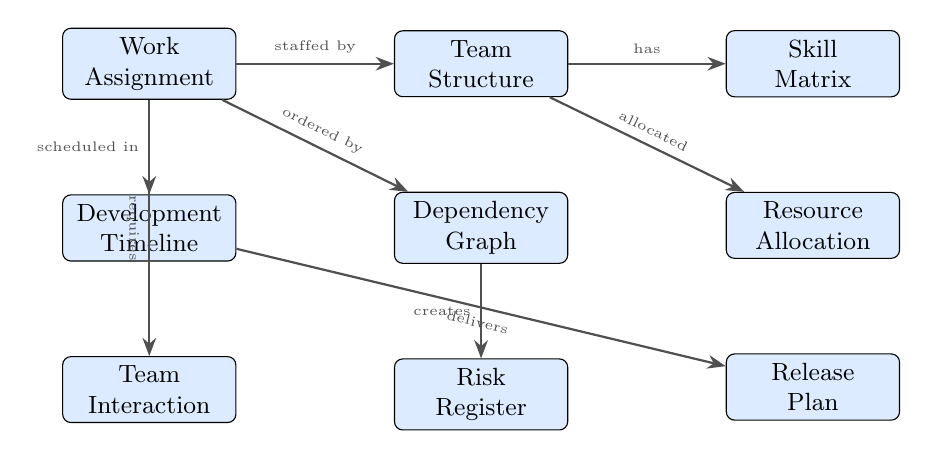
\begin{tikzpicture}[
    node distance=1.2cm and 2cm,
    model/.style={draw, fill=teamcolor, rounded corners=3pt, minimum width=2.2cm, minimum height=0.7cm, font=\small, align=center},
    arrow/.style={-{Stealth}, thick, darkgray}
]
    % Nodes - top row
    \node[model] (assignment) {Work\\Assignment};
    \node[model, right=2cm of assignment] (teams) {Team\\Structure};
    \node[model, right=2cm of teams] (skills) {Skill\\Matrix};
    
    % Nodes - middle row
    \node[model, below=1.2cm of assignment] (timeline) {Development\\Timeline};
    \node[model, below=1.2cm of teams] (depend) {Dependency\\Graph};
    \node[model, below=1.2cm of skills] (resource) {Resource\\Allocation};
    
    % Nodes - bottom row
    \node[model, below=1.2cm of timeline] (interact) {Team\\Interaction};
    \node[model, below=1.2cm of depend] (risk) {Risk\\Register};
    \node[model, below=1.2cm of resource] (release) {Release\\Plan};
    
    % Arrows
    \draw[arrow] (assignment) -- (teams) node[midway, above, font=\tiny] {staffed by};
    \draw[arrow] (teams) -- (skills) node[midway, above, font=\tiny] {has};
    \draw[arrow] (assignment) -- (timeline) node[midway, left, font=\tiny] {scheduled in};
    \draw[arrow] (assignment) -- (depend) node[midway, above, sloped, font=\tiny] {ordered by};
    \draw[arrow] (teams) -- (resource) node[midway, above, sloped, font=\tiny] {allocated};
    \draw[arrow] (depend) -- (risk) node[midway, left, font=\tiny] {creates};
    \draw[arrow] (assignment) -- (interact) node[midway, below, sloped, font=\tiny] {requires};
    \draw[arrow] (timeline) -- (release) node[midway, below, sloped, font=\tiny] {delivers};
\end{tikzpicture}
\caption{Model Type Dependency Relationships}
\end{figure}

% =============================================================================
% SECTION: MODEL LANGUAGES
% =============================================================================
\section{Model Languages}

For each model type, specific languages, notations, and techniques are prescribed.

\subsection{Work Assignment Notation}

\begin{figure}[H]
\centering
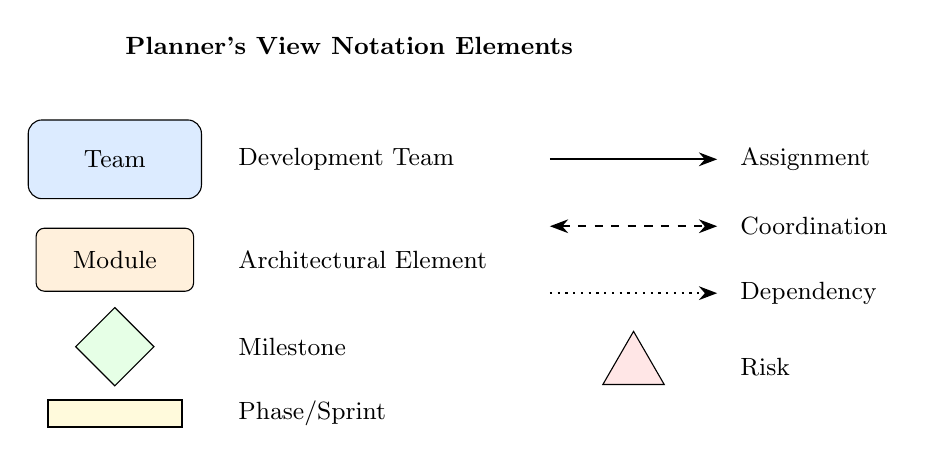
\begin{tikzpicture}[scale=0.85]
    % Legend title
    \node[font=\small\bfseries] at (0, 5) {Planner's View Notation Elements};
    
    % Team
    \node[draw, fill=teamcolor, rounded corners=5pt, minimum width=2.2cm, minimum height=1cm] at (-3.5, 3.3) {};
    \node[font=\small] at (-3.5, 3.3) {Team};
    \node[right, font=\small] at (-1.8, 3.3) {Development Team};
    
    % Module
    \node[draw, fill=modulecolor, rounded corners=3pt, minimum width=2cm, minimum height=0.8cm] at (-3.5, 1.8) {};
    \node[font=\small] at (-3.5, 1.8) {Module};
    \node[right, font=\small] at (-1.8, 1.8) {Architectural Element};
    
    % Milestone
    \node[draw, fill=milestonecolor, diamond, minimum size=1cm] at (-3.5, 0.5) {};
    \node[right, font=\small] at (-1.8, 0.5) {Milestone};
    
    % Phase
    \draw[thick, fill=phasecolor] (-4.5, -0.3) rectangle (-2.5, -0.7);
    \node[right, font=\small] at (-1.8, -0.5) {Phase/Sprint};
    
    % Dependency
    \draw[-{Stealth}, thick] (3, 3.3) -- (5.5, 3.3);
    \node[right, font=\small] at (5.7, 3.3) {Assignment};
    
    % Coordination
    \draw[{Stealth}-{Stealth}, thick, dashed] (3, 2.3) -- (5.5, 2.3);
    \node[right, font=\small] at (5.7, 2.3) {Coordination};
    
    % Dependency
    \draw[-{Stealth}, thick, dotted] (3, 1.3) -- (5.5, 1.3);
    \node[right, font=\small] at (5.7, 1.3) {Dependency};
    
    % Risk
    \node[draw, fill=riskcolor, regular polygon, regular polygon sides=3, minimum size=0.9cm] at (4.25, 0.2) {};
    \node[right, font=\small] at (5.7, 0.2) {Risk};
    
\end{tikzpicture}
\caption{Planner's View Notation Legend}
\end{figure}

\subsection{Team Topology Types}

\begin{table}[H]
\centering
\caption{Team Topology Classification (based on Team Topologies)}
\small
\begin{tabular}{@{}L{2.5cm}L{4.5cm}L{5.5cm}@{}}
\toprule
\textbf{Team Type} & \textbf{Description} & \textbf{Characteristics} \\
\midrule
Stream-Aligned & Aligned to flow of work for a business domain & End-to-end ownership, fast flow, autonomous \\
\addlinespace
Platform & Provides internal services to stream teams & Self-service, reduces cognitive load, enables \\
\addlinespace
Enabling & Helps other teams overcome obstacles & Temporary, consultative, capability building \\
\addlinespace
Complicated Subsystem & Handles complex specialized area & Deep expertise, shields complexity, specialist \\
\bottomrule
\end{tabular}
\end{table}

\subsection{Team Interaction Modes}

\begin{table}[H]
\centering
\caption{Team Interaction Mode Classification}
\small
\begin{tabular}{@{}L{2.5cm}L{4cm}L{6cm}@{}}
\toprule
\textbf{Mode} & \textbf{Description} & \textbf{When to Use} \\
\midrule
Collaboration & Close work together & Discovery, innovation, solving complex problems \\
\addlinespace
X-as-a-Service & One team provides, other consumes & Clear interface, platform capabilities \\
\addlinespace
Facilitating & One team helps another & Capability building, obstacle removal \\
\bottomrule
\end{tabular}
\end{table}

\subsection{Responsibility Assignment (RACI)}

\begin{table}[H]
\centering
\caption{RACI Responsibility Types}
\small
\begin{tabular}{@{}L{2.5cm}L{10cm}@{}}
\toprule
\textbf{Type} & \textbf{Description} \\
\midrule
Responsible (R) & Does the work. May be multiple people. \\
\addlinespace
Accountable (A) & Ultimately answerable. Only one person. \\
\addlinespace
Consulted (C) & Provides input before decisions. Two-way communication. \\
\addlinespace
Informed (I) & Kept up-to-date. One-way communication. \\
\bottomrule
\end{tabular}
\end{table}

\subsection{Tabular Specifications}

\subsubsection{Work Assignment Table}

\begin{table}[H]
\centering
\caption{Example Work Assignment Matrix}
\small
\begin{tabular}{@{}L{2.5cm}C{1.5cm}C{1.5cm}C{1.5cm}C{1.5cm}C{1.5cm}@{}}
\toprule
\textbf{Element} & \textbf{Team A} & \textbf{Team B} & \textbf{Team C} & \textbf{Platform} & \textbf{QA} \\
\midrule
Web Frontend & R/A & -- & C & C & C \\
Mobile App & R/A & -- & -- & C & C \\
Order Service & I & R/A & C & C & C \\
User Service & C & R/A & -- & C & C \\
API Gateway & C & C & R/A & R & C \\
Infrastructure & -- & -- & C & R/A & I \\
\bottomrule
\end{tabular}
\end{table}

\subsubsection{Team Specification Table}

\begin{table}[H]
\centering
\caption{Example Team Specification}
\small
\begin{tabular}{@{}L{2cm}L{2cm}C{1.2cm}L{3.5cm}L{3cm}@{}}
\toprule
\textbf{Team} & \textbf{Type} & \textbf{Size} & \textbf{Key Skills} & \textbf{Ownership} \\
\midrule
Alpha & Stream-Aligned & 6 & React, TypeScript, UX & Frontend, Mobile \\
\addlinespace
Beta & Stream-Aligned & 7 & Java, Spring, SQL & Orders, Users, Inventory \\
\addlinespace
Gamma & Complicated Subsystem & 4 & ML, Python, Data & Recommendations, Analytics \\
\addlinespace
Platform & Platform & 5 & K8s, AWS, Terraform & Infrastructure, CI/CD \\
\bottomrule
\end{tabular}
\end{table}

\subsubsection{Milestone Definition Table}

\begin{table}[H]
\centering
\caption{Example Milestone Definition}
\small
\begin{tabular}{@{}L{1.5cm}L{2.5cm}L{2cm}L{4cm}L{2.5cm}@{}}
\toprule
\textbf{ID} & \textbf{Milestone} & \textbf{Target} & \textbf{Deliverables} & \textbf{Criteria} \\
\midrule
M1 & Foundation & 2024-Q1 & Infrastructure, CI/CD, Auth & Env deployed, pipeline working \\
\addlinespace
M2 & Core MVP & 2024-Q2 & Orders, Users, Basic UI & E2E flow functional \\
\addlinespace
M3 & Beta Release & 2024-Q3 & Full features, Mobile & 100 beta users \\
\addlinespace
M4 & GA Release & 2024-Q4 & Production ready & Performance, security certified \\
\bottomrule
\end{tabular}
\end{table}

% =============================================================================
% SECTION: VIEWPOINT METAMODELS
% =============================================================================
\section{Viewpoint Metamodels}

This section defines the conceptual metamodel underlying the Planner's View.

\subsection{Core Metamodel}

\begin{figure}[H]
\centering
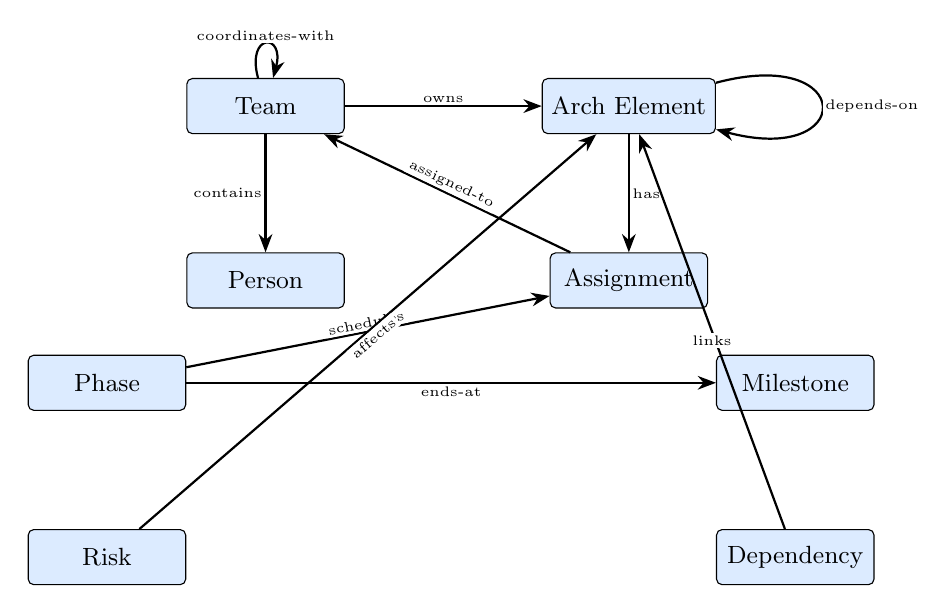
\begin{tikzpicture}[
    node distance=1.3cm and 2cm,
    entity/.style={draw, fill=teamcolor, rounded corners=2pt, minimum width=2cm, minimum height=0.7cm, font=\small},
    arrow/.style={-{Stealth}, thick},
    label/.style={font=\tiny, fill=white, inner sep=1pt}
]
    % Main entities
    \node[entity] (team) {Team};
    \node[entity, right=2.5cm of team] (element) {Arch Element};
    \node[entity, below=1.5cm of team] (person) {Person};
    \node[entity, below=1.5cm of element] (assignment) {Assignment};
    \node[entity, below left=2.8cm and 0cm of team] (phase) {Phase};
    \node[entity, below right=2.8cm and 0cm of element] (milestone) {Milestone};
    \node[entity, below=1.5cm of phase] (risk) {Risk};
    \node[entity, below=1.5cm of milestone] (dependency) {Dependency};
    
    % Relationships
    \draw[arrow] (team) -- (element) node[label, midway, above] {owns};
    \draw[arrow] (team) -- (person) node[label, midway, left] {contains};
    \draw[arrow] (element) -- (assignment) node[label, midway, right] {has};
    \draw[arrow] (assignment) -- (team) node[label, midway, above, sloped] {assigned-to};
    \draw[arrow] (phase) -- (assignment) node[label, midway, above, sloped] {schedules};
    \draw[arrow] (phase) -- (milestone) node[label, midway, below] {ends-at};
    \draw[arrow] (risk) -- (element) node[label, midway, below, sloped] {affects};
    \draw[arrow] (dependency) -- (element) node[label, midway, below] {links};
    
    % Self-reference
    \draw[arrow] (team) to[loop above] node[label, above] {coordinates-with} (team);
    \draw[arrow] (element) to[loop right] node[label, right] {depends-on} (element);
\end{tikzpicture}
\caption{Planner's View Core Metamodel}
\end{figure}

\subsection{Entity Definitions}

\begin{definitionbox}[Entity: Team]
\textbf{Definition:} An organizational unit consisting of people who work together to develop and maintain assigned architectural elements.

\textbf{Attributes:}
\begin{itemize}[nosep]
    \item \texttt{teamId}: Unique identifier
    \item \texttt{name}: Team name
    \item \texttt{description}: Team purpose and mission
    \item \texttt{type}: Team type (stream-aligned, platform, enabling, complicated subsystem)
    \item \texttt{size}: Number of team members
    \item \texttt{lead}: Team lead/manager
    \item \texttt{members}: List of team members
    \item \texttt{skills}: Collective skills and capabilities
    \item \texttt{capacity}: Available capacity (story points, hours)
    \item \texttt{location}: Physical/virtual location
    \item \texttt{timezone}: Primary timezone
\end{itemize}

\textbf{Constraints:}
\begin{itemize}[nosep]
    \item Team size should be 4-9 members (two-pizza rule)
    \item Team should have clear ownership of elements
    \item Skills should match assigned work
    \item Team should minimize external dependencies
\end{itemize}
\end{definitionbox}

\begin{definitionbox}[Entity: Architectural Element]
\textbf{Definition:} A component of the architecture that requires development effort and has assigned ownership.

\textbf{Attributes:}
\begin{itemize}[nosep]
    \item \texttt{elementId}: Unique identifier
    \item \texttt{name}: Element name
    \item \texttt{description}: Element purpose
    \item \texttt{type}: Element type (module, service, component, subsystem)
    \item \texttt{complexity}: Complexity rating
    \item \texttt{size}: Estimated size/effort
    \item \texttt{priority}: Development priority
    \item \texttt{status}: Current status
    \item \texttt{dependencies}: Elements this depends on
    \item \texttt{interfaces}: Interfaces with other elements
    \item \texttt{requiredSkills}: Skills needed to develop
\end{itemize}

\textbf{Constraints:}
\begin{itemize}[nosep]
    \item Element should have single owning team
    \item Dependencies should be explicit
    \item Size estimates should be provided
    \item Priority should be assigned
\end{itemize}
\end{definitionbox}

\begin{definitionbox}[Entity: Assignment]
\textbf{Definition:} The allocation of responsibility for an architectural element to a team, including the type and extent of responsibility.

\textbf{Attributes:}
\begin{itemize}[nosep]
    \item \texttt{assignmentId}: Unique identifier
    \item \texttt{element}: Assigned architectural element
    \item \texttt{team}: Responsible team
    \item \texttt{responsibilityType}: Type (R/A/C/I or owner/contributor)
    \item \texttt{startDate}: When assignment begins
    \item \texttt{endDate}: When assignment ends (if temporary)
    \item \texttt{effort}: Estimated effort required
    \item \texttt{allocation}: Percentage of team capacity
    \item \texttt{notes}: Additional assignment details
\end{itemize}

\textbf{Constraints:}
\begin{itemize}[nosep]
    \item Each element should have exactly one Accountable team
    \item Allocation should not exceed team capacity
    \item Temporary assignments should have end dates
\end{itemize}
\end{definitionbox}

\begin{definitionbox}[Entity: Person]
\textbf{Definition:} An individual contributor assigned to a team with specific skills and capacity.

\textbf{Attributes:}
\begin{itemize}[nosep]
    \item \texttt{personId}: Unique identifier
    \item \texttt{name}: Person's name
    \item \texttt{role}: Job role/title
    \item \texttt{team}: Primary team assignment
    \item \texttt{skills}: Individual skills and proficiency
    \item \texttt{availability}: Available hours/percentage
    \item \texttt{startDate}: When person joins project
    \item \texttt{endDate}: When person leaves (if known)
    \item \texttt{location}: Work location
    \item \texttt{timezone}: Personal timezone
\end{itemize}

\textbf{Constraints:}
\begin{itemize}[nosep]
    \item Person should have primary team assignment
    \item Skills should be documented
    \item Availability should be realistic
\end{itemize}
\end{definitionbox}

\begin{definitionbox}[Entity: Phase]
\textbf{Definition:} A distinct period in the project timeline with specific goals, activities, and deliverables.

\textbf{Attributes:}
\begin{itemize}[nosep]
    \item \texttt{phaseId}: Unique identifier
    \item \texttt{name}: Phase name
    \item \texttt{description}: Phase purpose and goals
    \item \texttt{startDate}: Phase start date
    \item \texttt{endDate}: Phase end date
    \item \texttt{milestone}: Ending milestone
    \item \texttt{deliverables}: Expected deliverables
    \item \texttt{activities}: Key activities in phase
    \item \texttt{exitCriteria}: Criteria to complete phase
    \item \texttt{risks}: Phase-specific risks
\end{itemize}

\textbf{Constraints:}
\begin{itemize}[nosep]
    \item Phases should not overlap
    \item Each phase should have clear exit criteria
    \item Deliverables should be measurable
\end{itemize}
\end{definitionbox}

\begin{definitionbox}[Entity: Milestone]
\textbf{Definition:} A significant point in the project timeline marking completion of a major deliverable or achievement.

\textbf{Attributes:}
\begin{itemize}[nosep]
    \item \texttt{milestoneId}: Unique identifier
    \item \texttt{name}: Milestone name
    \item \texttt{description}: Milestone significance
    \item \texttt{targetDate}: Planned date
    \item \texttt{actualDate}: Actual achievement date
    \item \texttt{deliverables}: What is delivered
    \item \texttt{criteria}: Success criteria
    \item \texttt{dependencies}: Predecessor milestones
    \item \texttt{status}: Status (planned, at-risk, achieved, missed)
    \item \texttt{owner}: Accountable person
\end{itemize}

\textbf{Constraints:}
\begin{itemize}[nosep]
    \item Milestones should have clear criteria
    \item Dependencies should be explicit
    \item Owner should be assigned
\end{itemize}
\end{definitionbox}

\begin{definitionbox}[Entity: Dependency]
\textbf{Definition:} A relationship where one work item requires another to be completed first.

\textbf{Attributes:}
\begin{itemize}[nosep]
    \item \texttt{dependencyId}: Unique identifier
    \item \texttt{predecessor}: Work item that must complete first
    \item \texttt{successor}: Work item that depends on predecessor
    \item \texttt{type}: Dependency type (finish-to-start, start-to-start, etc.)
    \item \texttt{lag}: Time lag between items
    \item \texttt{strength}: How critical (hard, soft, preference)
    \item \texttt{description}: Nature of dependency
    \item \texttt{risk}: Risk if dependency is not met
\end{itemize}

\textbf{Constraints:}
\begin{itemize}[nosep]
    \item Dependencies should be acyclic
    \item Critical dependencies should be highlighted
    \item Risk should be assessed for hard dependencies
\end{itemize}
\end{definitionbox}

\begin{definitionbox}[Entity: Risk]
\textbf{Definition:} A potential event or condition that could negatively impact project objectives.

\textbf{Attributes:}
\begin{itemize}[nosep]
    \item \texttt{riskId}: Unique identifier
    \item \texttt{name}: Risk name
    \item \texttt{description}: Risk description
    \item \texttt{category}: Risk category (technical, resource, schedule, external)
    \item \texttt{probability}: Likelihood (low, medium, high)
    \item \texttt{impact}: Potential impact (low, medium, high)
    \item \texttt{exposure}: Risk exposure (probability $\times$ impact)
    \item \texttt{affectedElements}: Elements affected
    \item \texttt{mitigation}: Mitigation strategy
    \item \texttt{contingency}: Contingency plan
    \item \texttt{owner}: Risk owner
    \item \texttt{status}: Current status
\end{itemize}

\textbf{Constraints:}
\begin{itemize}[nosep]
    \item High exposure risks must have mitigation plans
    \item Risks should have owners
    \item Status should be regularly updated
\end{itemize}
\end{definitionbox}

\subsection{Relationship Definitions}

\begin{table}[H]
\centering
\caption{Metamodel Relationship Definitions}
\small
\begin{tabular}{@{}L{2.3cm}L{1.8cm}L{1.8cm}L{7.5cm}@{}}
\toprule
\textbf{Relationship} & \textbf{Source} & \textbf{Target} & \textbf{Description} \\
\midrule
owns & Team & Element & Team is responsible for element \\
\addlinespace
contains & Team & Person & Team includes this person \\
\addlinespace
has & Element & Assignment & Element has this work assignment \\
\addlinespace
assigned-to & Assignment & Team & Assignment is given to team \\
\addlinespace
schedules & Phase & Assignment & Phase includes this work \\
\addlinespace
ends-at & Phase & Milestone & Phase concludes at milestone \\
\addlinespace
affects & Risk & Element & Risk impacts this element \\
\addlinespace
links & Dependency & Element & Dependency connects elements \\
\addlinespace
coordinates & Team & Team & Teams must coordinate \\
\addlinespace
depends-on & Element & Element & Element requires another \\
\bottomrule
\end{tabular}
\end{table}

% =============================================================================
% SECTION: CONFORMING NOTATIONS
% =============================================================================
\section{Conforming Notations}

Several existing notations and tools support Planner's View modeling.

\subsection{Gantt Charts}

Gantt charts are the most common notation for project timeline visualization.

\textbf{Elements:} Tasks, durations, dependencies, milestones, resources.

\textbf{Tool Support:} Microsoft Project, Smartsheet, GanttPro, Jira.

\textbf{Conformance Level:} High for timeline, medium for architecture mapping.

\subsection{Network Diagrams (PERT/CPM)}

Network diagrams show activity dependencies and critical path.

\textbf{Elements:} Activities, dependencies, durations, slack.

\textbf{Analysis:} Critical path, float time, earliest/latest dates.

\textbf{Conformance Level:} High for dependency analysis.

\subsection{Team Topologies Notation}

Team Topologies provides notation for team structure and interactions.

\textbf{Elements:} Team types, interaction modes, cognitive load.

\textbf{Tool Support:} Team Topologies diagrams, Miro templates.

\textbf{Conformance Level:} High for team structure modeling.

\subsection{Design Structure Matrix (DSM)}

DSM shows dependencies between elements in matrix form.

\textbf{Elements:} Elements, dependencies (marked cells).

\textbf{Analysis:} Clustering, partitioning, tearing.

\textbf{Conformance Level:} High for dependency and coordination analysis.

\subsection{Notation Comparison}

\begin{table}[H]
\centering
\caption{Planning Notation Comparison}
\small
\begin{tabular}{@{}L{2.5cm}C{1.2cm}C{1.2cm}C{1.2cm}C{1.2cm}C{1.2cm}C{1.2cm}@{}}
\toprule
\textbf{Feature} & \rotatebox{60}{\textbf{Gantt}} & \rotatebox{60}{\textbf{PERT}} & \rotatebox{60}{\textbf{DSM}} & \rotatebox{60}{\textbf{RACI}} & \rotatebox{60}{\textbf{Team Top.}} & \rotatebox{60}{\textbf{Roadmap}} \\
\midrule
Timeline & $\bullet$ & $\circ$ & -- & -- & -- & $\bullet$ \\
Dependencies & $\circ$ & $\bullet$ & $\bullet$ & -- & $\circ$ & $\circ$ \\
Resources & $\bullet$ & $\circ$ & -- & $\bullet$ & $\circ$ & -- \\
Milestones & $\bullet$ & $\bullet$ & -- & -- & -- & $\bullet$ \\
Team structure & $\circ$ & -- & $\circ$ & $\circ$ & $\bullet$ & -- \\
Coordination & -- & -- & $\bullet$ & $\circ$ & $\bullet$ & -- \\
Work assignment & $\circ$ & -- & $\circ$ & $\bullet$ & $\circ$ & -- \\
\bottomrule
\multicolumn{7}{l}{\footnotesize $\bullet$ = Strong support, $\circ$ = Limited support, -- = Not applicable}
\end{tabular}
\end{table}

% =============================================================================
% SECTION: MODEL CORRESPONDENCE RULES
% =============================================================================
\section{Model Correspondence Rules}

Model correspondence rules define how elements in planner's models relate to elements in other architectural views.

\subsection{Development View Correspondence}

\begin{definitionbox}[Correspondence Rule CR-01: Module to Team Mapping]
\textbf{Rule:} Every code module should have an owning team assignment.

\textbf{Formal Expression:}
\begin{center}
$\forall m \in Modules : \exists t \in Teams : owns(t, m)$
\end{center}

\textbf{Rationale:} Ensures clear ownership and accountability for code.

\textbf{Verification:} Module ownership matrix review.
\end{definitionbox}

\begin{definitionbox}[Correspondence Rule CR-02: Package Alignment]
\textbf{Rule:} Package structure should align with team boundaries where possible.

\textbf{Formal Expression:}
\begin{center}
$packages(team_1) \cap packages(team_2) \approx \emptyset$
\end{center}

\textbf{Rationale:} Reduces coordination overhead (Conway's Law).

\textbf{Verification:} Package-to-team mapping review.
\end{definitionbox}

\subsection{Logical View Correspondence}

\begin{definitionbox}[Correspondence Rule CR-03: Domain to Team Mapping]
\textbf{Rule:} Bounded contexts should map to team ownership.

\textbf{Formal Expression:}
\begin{center}
$\forall bc \in BoundedContexts : \exists t \in Teams : owns(t, bc)$
\end{center}

\textbf{Rationale:} Aligns team structure with domain structure (inverse Conway).

\textbf{Verification:} Domain-to-team mapping review.
\end{definitionbox}

\subsection{Component-and-Connector View Correspondence}

\begin{definitionbox}[Correspondence Rule CR-04: Interface to Coordination]
\textbf{Rule:} Interfaces between components owned by different teams require coordination.

\textbf{Formal Expression:}
\begin{center}
$\forall i \in Interfaces : owner(source(i)) \neq owner(target(i)) \Rightarrow coordinates(owner(source(i)), owner(target(i)))$
\end{center}

\textbf{Rationale:} Ensures necessary team coordination is planned.

\textbf{Verification:} Team interaction matrix completeness.
\end{definitionbox}

% =============================================================================
% SECTION: OPERATIONS ON VIEWS
% =============================================================================
\section{Operations on Views}

This section defines methods for creating, interpreting, analyzing, and maintaining planner's views.

\subsection{Creation Methods}

\subsubsection{View Development Process}

\begin{guidancebox}[Step 1: Identify Architectural Elements]
\begin{enumerate}[nosep]
    \item Extract elements from development/logical views
    \item Determine granularity for assignment
    \item Identify element dependencies
    \item Estimate element complexity and size
    \item Prioritize elements for development
\end{enumerate}
\end{guidancebox}

\begin{guidancebox}[Step 2: Define Team Structure]
\begin{enumerate}[nosep]
    \item Determine required team types
    \item Size teams appropriately (5-9 members)
    \item Identify required skills per team
    \item Assign team leads
    \item Define team missions and boundaries
\end{enumerate}
\end{guidancebox}

\begin{guidancebox}[Step 3: Create Work Assignments]
\begin{enumerate}[nosep]
    \item Map elements to teams
    \item Assign RACI responsibilities
    \item Balance workload across teams
    \item Identify skill gaps
    \item Document assignment rationale
\end{enumerate}
\end{guidancebox}

\begin{guidancebox}[Step 4: Sequence Development]
\begin{enumerate}[nosep]
    \item Analyze architectural dependencies
    \item Identify critical path
    \item Determine parallel work opportunities
    \item Plan integration points
    \item Create dependency graph
\end{enumerate}
\end{guidancebox}

\begin{guidancebox}[Step 5: Define Phases and Milestones]
\begin{enumerate}[nosep]
    \item Identify major project phases
    \item Define milestones and criteria
    \item Allocate work to phases
    \item Set target dates
    \item Plan deliverables per phase
\end{enumerate}
\end{guidancebox}

\begin{guidancebox}[Step 6: Plan Team Coordination]
\begin{enumerate}[nosep]
    \item Identify inter-team interfaces
    \item Define coordination mechanisms
    \item Plan integration activities
    \item Schedule synchronization points
    \item Document communication protocols
\end{enumerate}
\end{guidancebox}

\begin{guidancebox}[Step 7: Assess and Mitigate Risks]
\begin{enumerate}[nosep]
    \item Identify technical and organizational risks
    \item Assess probability and impact
    \item Develop mitigation strategies
    \item Create contingency plans
    \item Assign risk owners
\end{enumerate}
\end{guidancebox}

\subsubsection{Team Organization Patterns}

\begin{patternbox}[Pattern: Stream-Aligned Teams]
\textbf{Context:} Need fast flow of features to production.

\textbf{Solution:} Organize teams around end-to-end value streams.

\textbf{Characteristics:}
\begin{itemize}[nosep]
    \item Full ownership from idea to production
    \item Cross-functional (dev, test, ops skills)
    \item Aligned with business domain
    \item Minimized handoffs
\end{itemize}

\textbf{Use When:} Optimizing for delivery speed and autonomy.
\end{patternbox}

\begin{patternbox}[Pattern: Platform Teams]
\textbf{Context:} Multiple teams need common capabilities.

\textbf{Solution:} Dedicated team provides self-service platform.

\textbf{Characteristics:}
\begin{itemize}[nosep]
    \item Provides infrastructure, tools, capabilities
    \item Self-service consumption model
    \item Reduces cognitive load on stream teams
    \item Enables rather than gates
\end{itemize}

\textbf{Use When:} Shared infrastructure or capabilities needed.
\end{patternbox}

\begin{patternbox}[Pattern: Inverse Conway Maneuver]
\textbf{Context:} Architecture and team structure misaligned.

\textbf{Solution:} Restructure teams to match desired architecture.

\textbf{Characteristics:}
\begin{itemize}[nosep]
    \item Architecture drives team structure
    \item Teams own bounded contexts
    \item Clear interfaces between teams
    \item Reduced coordination overhead
\end{itemize}

\textbf{Use When:} Designing new architecture, restructuring organization.
\end{patternbox}

\subsection{Analysis Methods}

\subsubsection{Critical Path Analysis}

\begin{definitionbox}[Critical Path Method (CPM)]
\textbf{Purpose:} Identify the longest sequence of dependent activities.

\textbf{Process:}
\begin{enumerate}[nosep]
    \item List all activities and durations
    \item Identify dependencies
    \item Calculate forward pass (earliest start/finish)
    \item Calculate backward pass (latest start/finish)
    \item Identify zero-float activities (critical path)
\end{enumerate}

\textbf{Output:} Critical path, activity float, project duration.

\textbf{Application:} Focus resources on critical path activities.
\end{definitionbox}

\subsubsection{Team Dependency Analysis}

\begin{definitionbox}[Team Interaction Assessment]
\textbf{Purpose:} Analyze coordination requirements between teams.

\textbf{Factors:}
\begin{itemize}[nosep]
    \item Number of shared interfaces
    \item Frequency of coordination needed
    \item Synchronization requirements
    \item Communication overhead
\end{itemize}

\textbf{Output:} Team interaction matrix with coordination intensity.

\textbf{Application:} Identify high-coordination pairs for attention.
\end{definitionbox}

% =============================================================================
% SECTION: EXAMPLES
% =============================================================================
\section{Examples}

\subsection{Example 1: Work Assignment Diagram}

\begin{figure}[H]
\centering
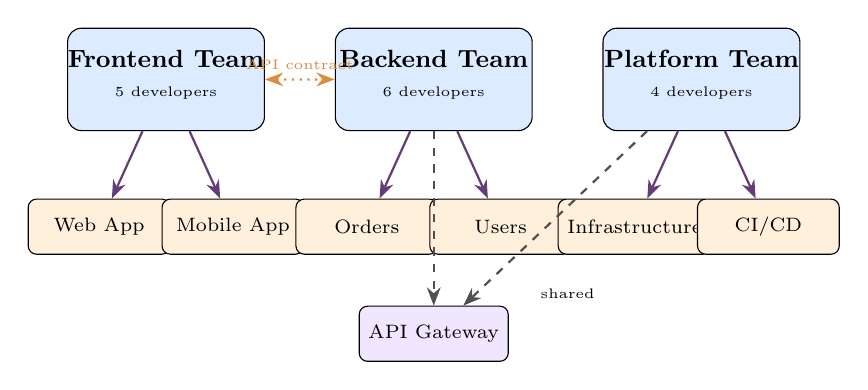
\begin{tikzpicture}[
    team/.style={draw, fill=teamcolor, rounded corners=5pt, minimum width=2.5cm, minimum height=1.3cm},
    module/.style={draw, fill=modulecolor, rounded corners=3pt, minimum width=1.8cm, minimum height=0.7cm, font=\scriptsize},
    scale=0.85
]
    % Teams
    \node[team] (frontend) at (-4, 3) {};
    \node[font=\small\bfseries] at (-4, 3.3) {Frontend Team};
    \node[font=\tiny] at (-4, 2.8) {5 developers};
    
    \node[team] (backend) at (0, 3) {};
    \node[font=\small\bfseries] at (0, 3.3) {Backend Team};
    \node[font=\tiny] at (0, 2.8) {6 developers};
    
    \node[team] (platform) at (4, 3) {};
    \node[font=\small\bfseries] at (4, 3.3) {Platform Team};
    \node[font=\tiny] at (4, 2.8) {4 developers};
    
    % Modules
    \node[module] (web) at (-5, 0.8) {Web App};
    \node[module] (mobile) at (-3, 0.8) {Mobile App};
    
    \node[module] (orders) at (-1, 0.8) {Orders};
    \node[module] (users) at (1, 0.8) {Users};
    
    \node[module] (infra) at (3, 0.8) {Infrastructure};
    \node[module] (cicd) at (5, 0.8) {CI/CD};
    
    % Shared module
    \node[module, fill=dependcolor] (api) at (0, -0.8) {API Gateway};
    
    % Assignments
    \draw[-{Stealth}, thick, primary] (frontend) -- (web);
    \draw[-{Stealth}, thick, primary] (frontend) -- (mobile);
    \draw[-{Stealth}, thick, primary] (backend) -- (orders);
    \draw[-{Stealth}, thick, primary] (backend) -- (users);
    \draw[-{Stealth}, thick, primary] (platform) -- (infra);
    \draw[-{Stealth}, thick, primary] (platform) -- (cicd);
    
    % Shared ownership
    \draw[-{Stealth}, thick, dashed, darkgray] (backend) -- (api);
    \draw[-{Stealth}, thick, dashed, darkgray] (platform) -- (api);
    \node[font=\tiny] at (2, -0.2) {shared};
    
    % Coordination
    \draw[{Stealth}-{Stealth}, thick, dotted, accent] (frontend) -- (backend) node[midway, above, font=\tiny] {API contract};
    
\end{tikzpicture}
\caption{Work Assignment Diagram}
\end{figure}

\textbf{Description:} This diagram shows three teams with their assigned modules. Frontend Team owns Web and Mobile apps. Backend Team owns Orders and Users services. Platform Team owns Infrastructure and CI/CD. The API Gateway is shared between Backend and Platform teams. A coordination relationship exists between Frontend and Backend teams for API contracts.

\subsection{Example 2: Development Timeline}

\begin{figure}[H]
\centering
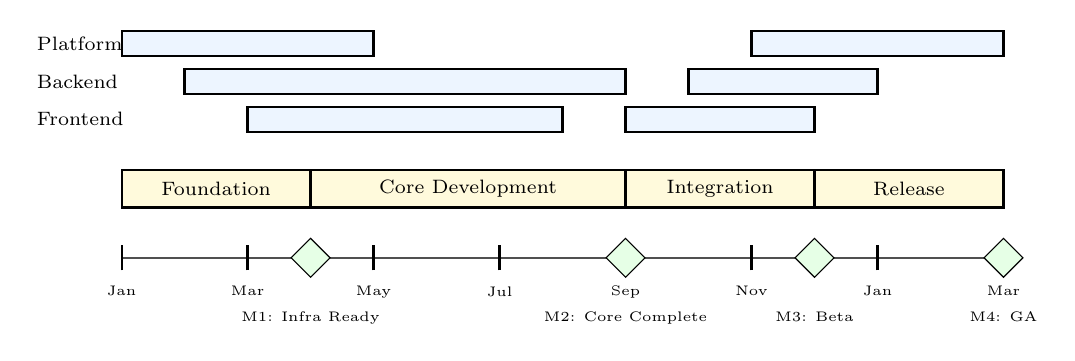
\begin{tikzpicture}[scale=0.8]
    % Timeline
    \draw[thick, darkgray] (0, 0) -- (14, 0);
    
    % Month markers
    \foreach \x/\month in {0/Jan, 2/Mar, 4/May, 6/Jul, 8/Sep, 10/Nov, 12/Jan, 14/Mar} {
        \draw[thick] (\x, -0.2) -- (\x, 0.2);
        \node[font=\tiny, below] at (\x, -0.3) {\month};
    }
    
    % Phases
    \draw[thick, fill=phasecolor] (0, 0.8) rectangle (3, 1.4);
    \node[font=\scriptsize] at (1.5, 1.1) {Foundation};
    
    \draw[thick, fill=phasecolor] (3, 0.8) rectangle (8, 1.4);
    \node[font=\scriptsize] at (5.5, 1.1) {Core Development};
    
    \draw[thick, fill=phasecolor] (8, 0.8) rectangle (11, 1.4);
    \node[font=\scriptsize] at (9.5, 1.1) {Integration};
    
    \draw[thick, fill=phasecolor] (11, 0.8) rectangle (14, 1.4);
    \node[font=\scriptsize] at (12.5, 1.1) {Release};
    
    % Team tracks
    \node[font=\scriptsize, right] at (-1.5, 2.2) {Frontend};
    \draw[thick, fill=teamcolor!50] (2, 2) rectangle (7, 2.4);
    \draw[thick, fill=teamcolor!50] (8, 2) rectangle (11, 2.4);
    
    \node[font=\scriptsize, right] at (-1.5, 2.8) {Backend};
    \draw[thick, fill=teamcolor!50] (1, 2.6) rectangle (8, 3);
    \draw[thick, fill=teamcolor!50] (9, 2.6) rectangle (12, 3);
    
    \node[font=\scriptsize, right] at (-1.5, 3.4) {Platform};
    \draw[thick, fill=teamcolor!50] (0, 3.2) rectangle (4, 3.6);
    \draw[thick, fill=teamcolor!50] (10, 3.2) rectangle (14, 3.6);
    
    % Milestones
    \node[draw, fill=milestonecolor, diamond, minimum size=0.5cm] at (3, 0) {};
    \node[font=\tiny, below] at (3, -0.7) {M1: Infra Ready};
    
    \node[draw, fill=milestonecolor, diamond, minimum size=0.5cm] at (8, 0) {};
    \node[font=\tiny, below] at (8, -0.7) {M2: Core Complete};
    
    \node[draw, fill=milestonecolor, diamond, minimum size=0.5cm] at (11, 0) {};
    \node[font=\tiny, below] at (11, -0.7) {M3: Beta};
    
    \node[draw, fill=milestonecolor, diamond, minimum size=0.5cm] at (14, 0) {};
    \node[font=\tiny, below] at (14, -0.7) {M4: GA};
    
\end{tikzpicture}
\caption{Development Timeline with Team Tracks}
\end{figure}

\textbf{Description:} This timeline shows the project phases (Foundation, Core Development, Integration, Release) with team activity tracks. Platform Team is active early for infrastructure and late for production readiness. Backend Team has the longest development phase. Frontend Team starts after API design and completes during integration. Milestones mark key completion points.

\subsection{Example 3: Risk Register}

\begin{table}[H]
\centering
\caption{Sample Risk Register}
\footnotesize
\begin{tabular}{@{}L{0.5cm}L{2.5cm}C{1cm}C{1cm}C{1cm}L{3cm}L{2cm}@{}}
\toprule
\textbf{ID} & \textbf{Risk} & \textbf{Prob.} & \textbf{Impact} & \textbf{Exp.} & \textbf{Mitigation} & \textbf{Owner} \\
\midrule
R1 & Key developer leaves & \cellcolor{yellow!30}Med & \cellcolor{red!30}High & \cellcolor{orange!30}High & Cross-training, documentation & Dev Manager \\
\addlinespace
R2 & External API delayed & \cellcolor{yellow!30}Med & \cellcolor{yellow!30}Med & \cellcolor{yellow!30}Med & Build mock, parallel dev & Architect \\
\addlinespace
R3 & Performance issues & \cellcolor{green!30}Low & \cellcolor{red!30}High & \cellcolor{yellow!30}Med & Early perf testing, budgets & Tech Lead \\
\addlinespace
R4 & Scope creep & \cellcolor{red!30}High & \cellcolor{yellow!30}Med & \cellcolor{orange!30}High & Change control, PM rigor & PM \\
\bottomrule
\end{tabular}
\end{table}

% =============================================================================
% SECTION: NOTES
% =============================================================================
\section{Notes}

\subsection{Conway's Law Considerations}

\begin{planningbox}[Conway's Law]
``Organizations which design systems are constrained to produce designs which are copies of the communication structures of these organizations.'' -- Melvin Conway, 1967

\textbf{Implications for Planning:}
\begin{itemize}[nosep]
    \item Architecture and team structure influence each other
    \item Align teams with desired architectural boundaries
    \item Reduce interfaces between teams to reduce component interfaces
    \item Use ``Inverse Conway Maneuver'' to drive architecture through team design
    \item Cross-team interfaces require coordination overhead
\end{itemize}
\end{planningbox}

\subsection{Estimation Guidelines}

\begin{teambox}[Estimation Best Practices]
\begin{itemize}[nosep]
    \item Use relative sizing (story points) for comparison
    \item Include uncertainty ranges (optimistic/expected/pessimistic)
    \item Account for unknowns with contingency
    \item Re-estimate as understanding improves
    \item Track actuals vs estimates for calibration
    \item Involve the team doing the work
    \item Consider dependencies in estimates
    \item Factor in integration and testing time
\end{itemize}
\end{teambox}

\subsection{Common Pitfalls}

\begin{warningbox}[Common Mistakes to Avoid]
\begin{enumerate}[nosep]
    \item \textbf{Ignoring Conway's Law:} Misaligned teams and architecture
    \item \textbf{Over-allocation:} Assigning more work than capacity allows
    \item \textbf{Hidden Dependencies:} Missing coordination requirements
    \item \textbf{Single Points of Failure:} Critical knowledge in one person
    \item \textbf{Optimistic Estimation:} Not accounting for uncertainty
    \item \textbf{Waterfall in Disguise:} Big-bang integration at end
    \item \textbf{Skill Mismatch:} Assigning work without needed skills
    \item \textbf{Communication Overhead:} Too many cross-team interfaces
\end{enumerate}
\end{warningbox}

% =============================================================================
% SECTION: SOURCES
% =============================================================================
\section{Sources}

\subsection{Primary References}

\begin{enumerate}
    \item Clements, P., et al. (2010). \textit{Documenting Software Architectures: Views and Beyond} (2nd ed.). Addison-Wesley Professional.
    
    \item Skelton, M., \& Pais, M. (2019). \textit{Team Topologies: Organizing Business and Technology Teams for Fast Flow}. IT Revolution Press.
    
    \item Conway, M. (1968). ``How Do Committees Invent?'' \textit{Datamation}, 14(4), 28-31.
    
    \item Bass, L., Clements, P., \& Kazman, R. (2021). \textit{Software Architecture in Practice} (4th ed.). Addison-Wesley Professional.
    
    \item Brooks, F. (1995). \textit{The Mythical Man-Month} (Anniversary ed.). Addison-Wesley Professional.
\end{enumerate}

\subsection{Supplementary References}

\begin{enumerate}[resume]
    \item McConnell, S. (2006). \textit{Software Estimation: Demystifying the Black Art}. Microsoft Press.
    
    \item DeMarco, T., \& Lister, T. (2013). \textit{Peopleware} (3rd ed.). Addison-Wesley Professional.
    
    \item Forsgren, N., Humble, J., \& Kim, G. (2018). \textit{Accelerate}. IT Revolution Press.
    
    \item Reinertsen, D. (2009). \textit{The Principles of Product Development Flow}. Celeritas Publishing.
    
    \item PMI. (2021). \textit{A Guide to the Project Management Body of Knowledge} (7th ed.).
\end{enumerate}

\subsection{Online Resources}

\begin{itemize}
    \item Team Topologies: \url{https://teamtopologies.com/}
    \item Agile Estimation: \url{https://www.mountaingoatsoftware.com/}
    \item Conway's Law: \url{https://www.melconway.com/Home/Conways_Law.html}
    \item DORA Research: \url{https://dora.dev/}
\end{itemize}

% =============================================================================
% APPENDIX
% =============================================================================
\appendix

\section{Planner's View Checklist}

\begin{table}[H]
\centering
\small
\begin{tabular}{@{}L{10cm}C{2cm}@{}}
\toprule
\textbf{Item} & \textbf{Complete?} \\
\midrule
\multicolumn{2}{l}{\textbf{Work Assignment}} \\
\quad All architectural elements have owners & $\square$ \\
\quad RACI responsibilities defined & $\square$ \\
\quad Workload balanced across teams & $\square$ \\
\quad Assignment rationale documented & $\square$ \\
\midrule
\multicolumn{2}{l}{\textbf{Team Structure}} \\
\quad Teams appropriately sized & $\square$ \\
\quad Team types defined (stream, platform, etc.) & $\square$ \\
\quad Skills match assignments & $\square$ \\
\quad Team leads identified & $\square$ \\
\midrule
\multicolumn{2}{l}{\textbf{Timeline}} \\
\quad Phases defined with criteria & $\square$ \\
\quad Milestones identified & $\square$ \\
\quad Critical path analyzed & $\square$ \\
\quad Dependencies mapped & $\square$ \\
\midrule
\multicolumn{2}{l}{\textbf{Coordination}} \\
\quad Inter-team interfaces identified & $\square$ \\
\quad Coordination mechanisms defined & $\square$ \\
\quad Integration points planned & $\square$ \\
\quad Communication protocols documented & $\square$ \\
\midrule
\multicolumn{2}{l}{\textbf{Risk Management}} \\
\quad Risks identified and assessed & $\square$ \\
\quad Mitigations defined & $\square$ \\
\quad Risk owners assigned & $\square$ \\
\quad Contingency plans created & $\square$ \\
\bottomrule
\end{tabular}
\end{table}

\section{Glossary}

\begin{description}[style=nextline, leftmargin=3cm, labelwidth=2.8cm]
    \item[Allocation] Assignment of resources to work items.
    
    \item[Capacity] Available work capacity of a team or person.
    
    \item[Conway's Law] Principle that system design mirrors organization structure.
    
    \item[Critical Path] Longest sequence of dependent activities.
    
    \item[Dependency] Relationship where one item requires another.
    
    \item[Float/Slack] Time an activity can be delayed without affecting schedule.
    
    \item[Milestone] Significant point marking project progress.
    
    \item[Phase] Distinct period with specific goals and activities.
    
    \item[Platform Team] Team providing shared capabilities to other teams.
    
    \item[RACI] Responsibility matrix (Responsible, Accountable, Consulted, Informed).
    
    \item[Stream-Aligned] Team aligned to business value stream.
    
    \item[Team Topology] Pattern for organizing teams.
    
    \item[Work Assignment] Allocation of architectural element to team.
    
    \item[Work Breakdown] Decomposition of work into assignable units.
\end{description}

% =============================================================================
% END DOCUMENT
% =============================================================================

\end{document}
